\documentclass[11pt,a4paper]{article}
\usepackage[utf8]{inputenc}
\usepackage{amsmath}
\usepackage{amsfonts}
\usepackage{amssymb}
\usepackage{multicol}
\usepackage{graphicx}
\usepackage{multicol}
\newcommand{\ds}{\displaystyle}
\pagestyle{empty}
\usepackage[left=2.00cm, right=2.00cm, top=2.00cm, bottom=2.00cm]{geometry}
\usepackage[usenames]{color}
\begin{document}
\begin{center}
\LARGE \noindent UNIVERSIDAD NACIONAL DE INGENIERÍA\\
Facultad de Ciencias\\
Matemática y Ciencia de La computaci{\'o}n
\end{center}
\begin{center}
\begin{minipage}[c]{9cm}

\includegraphics[scale=1.00]{uni.PNG}
\end{minipage}
\end{center}
\begin{center}
\Large \textbf{T{\'I}TULO DEL TRABAJO}\\
Verificaci{\'o}n de la existencia de un ciclo hamiltoniano en un grafo aleatorio
\end{center}
\begin{center}
\Large \textbf{Unidad Acad{\'e}mica}: 
\\Facultad de Ciencias\\
\textbf{Curso y secci{\'o}n}: 
\\Introducci{\'o}n a la Estad{\'i}stica\\ y Probabilidades(CM-274 "A")\\
\textbf{Semestre}: 
\\2018-II\\
\textbf{Profesores}:
\\ Zamudio Fernando - C{\'e}sar Lara\\
\textbf{Integrantes}:\\
/Jaafar Farut Sahua Torres/\\
/Franklin F{\'e}lix Rivera Granados/\\
/Briguitte Stefany Maquera de la Cruz/\\
\end{center}
\begin{center}
\LARGE \vfill\textbf{Lima-Per{\'u}}\\
\textbf{(2018)}
\end{center}

\begin{center}
\LARGE \textbf{\textcolor{blue}{Introducci{\'o}n}}\\[1cm]
\end{center}
\Large
\begin{multicols}{2}
\textbf{¿\underline{Qu{\'e} es un Grafo}?}\\
• \textbf{Grafo}: Es un diagrama que representa mediante vertices y aristas las relaciones entre pares de elementos y que se usa para resolver problemas l{\'o}gicos, topol{\'o}gicos y de c{\'a}lculo combinatorio.\\
• \textbf{Grafo hamiltoniano}: Es aquel grafo que tiene un ciclo hamiltoniano el cual recorre una sola vez cada vertice y el vertice final sea adyacente al primero, de esa forma contiene un camino hamiltoniano o circuito hamiltoniano.\\
\textbf{¿\underline{C{\'o}mo identificar un}}\\
\textbf{\underline{grafo hamiltoniano}?}\\
Contrario al caso de los grafos eulerianos, para el caso de los grafos hamiltonianos no se conoce ninguna condici{\'o}n necesaria y suficiente que los caracterice. Esto es lamentable porque en muchas aplicaciones es fundamental poder determinar si un grafo es hamiltoniano.\\
\textit{\textbf{Ejemplos de Grafos hamiltonianos}}\\
\begin{minipage}[c]{4cm}
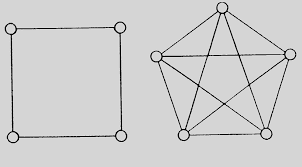
\includegraphics[scale=0.42]{grafo.PNG}
\end{minipage}\\[1cm]
\textbf{¿\underline{Qu{\'e} es el Lenguaje}}\\
\textbf{\underline{de programaci{\'o}n R}?}\\
Es un tipo de lenguaje de programaci{\'o}n el cual es una implementaci{\'o}n del lenguaje de programaci{\'o}n S, creado en Auckland(New Zealand)\\
•\textbf{Caracter{\'i}sticas}\\
\textbf{*} R es un lenguaje pensado para la programaci{\'o}n estad{\'i}stica y la creaci{\'o}n de gr{\'a}ficos\\
\textbf{*} Posee mucho paquetes y librerias\\
\textbf{*} Es multi-paradigm{\'a}tico y Open Source ya que nos permite una facilidad en el uso de la escritura o implementaci{\'o}n del c{\'o}digo\\
\textit{\textbf{Nota:}}RStudio es un entorno de desarrollo integrado (IDE) para el lenguaje de programación R, dedicado a la computación estadística y gráficos.\\
\begin{minipage}[c]{4cm}

\includegraphics[scale=0.41]{R.PNG}
\end{minipage}
\end{multicols}

\begin{center}
\LARGE \textbf{\textcolor{blue}{Objetivo del Proyecto}}\\[1cm]
\end{center}
\Large
\begin{multicols}{2}
• Es la verificaci{\'o}n de un grafo y determinar si es o no es hamiltoniano  pues ya que aunque no hay condici{\'o}n o formula totalmente eficiente para su demostracion, podemos aproximarnos utilizando ciertas condiciones.\\
• El implemento de la programacion mediante el uso del Lenguaje R en nuestro proyecto para dicha verificacion\\
• El uso de algunas formulas y teoremas estadisticos para la determinaci{\'o}n de un grafo y verificar si es o no es hamiltoniano\\[5cm]
\end{multicols}

\begin{center}
\LARGE \textbf{\textcolor{blue}{Estado del arte}}\\[1cm]
\end{center}
\Large
\begin{enumerate}
\begin{multicols}{2}
\item \textbf{Libro(PDF):}Matem{\'a}tica Discreta "Teoria de Grafos"\\
\textbf{autores:} Merce Claverol, Ester Simo y Marisa Zaragoza\\
\textbf{Tema 2:} p{\'a}ginas(38-39)\\[1cm]
• Este art{\'i}culo nos permiti{\'o} un analisi mas profundo sobre las carateristicas y formas de los grafos hamiltonianos\\
\item \textbf{Libro(PDF):} Teorema de Dirac y Ore (aplicaciones de la matetica discreta en la vide real)\\[1cm]
• Este art{\'i}culo nos permiti{\'o} un mejor an{\'a}lisis de los teoremas de Dirac y Ore, loscuales nos permiten la verificacion de un grafo y descubrir si es o no es hamiltoniano\\ 
\textbf{autores:} Alberto Conejero y Cristian J{\'o}rdan\\[1cm]  
\item \textbf{Video(Tutorial):}Introducci{\'o}n a los Grafos con igraph\\[1cm]
• Este tutorial nos permiti{\'o} una mejor visualizacion respecto a lo que ser{\'a} cuando aplicamos grafos en Lenguaje R\\
\item \textbf{Network Analysis and Visualization with R and igraph}\\[1cm]
• This page gave us information about the various functions that we can use in Rstudio and also about the igraph package which will help us in the graph drawings in Rstudio
\end{multicols}
\end{enumerate}

\begin{center}
\textbf{\textcolor{blue}{Diseño del experimento}}\\
\end{center}
\end{document}